\documentclass[a4paper]{article}

\usepackage[english]{babel}
\usepackage[utf8]{inputenc}
\usepackage{amsmath}
\usepackage{graphicx}
\usepackage{color}
\usepackage[colorinlistoftodos]{todonotes}

\title{Report Practical assignment 1}

\author{Machinists:\\
Fares Ben Slimane}

\date{\today}

\begin{document}
\maketitle

\begin{abstract}
This report explain our approaches to solving the problems of the practical assignment 1. the experiments we performed, results and conclusion of our work.
\end{abstract}

\section{Problem 1 (MLP)}
\label{sec:problem1}

\subsection{Building model}

\begin{enumerate}
  \item (using the python script mlp.py under the folder problem1), we build an MLP with two hidden layers h1(24 hidden units) and h2(12 hidden units).The total number of parameters of the network $= 784*512 + 512 + 512*1024 + 1024 + 1024*10 + 10 = 937,482 \approx 0.9 M$.
  
  \item We Implemented the forward and backward propagation in a generalized way (can work in any number of layers) of the MLP in numpy without the use of a deep learning framework and using the provided class structure. (See python script mlp.py under problem 1 folder).
  
  \item We trained the MLP using the probability loss (cross entropy) as training criterion (See loss method in the NN class) and minimize this criterion to optimize the model parameters using stochastic gradient descent (See the update method in the NN class). (See python script mlp.py under problem 1 folder).
  
\end{enumerate}

\subsection{Initialization}
We consider a model architecture of two hidden layers h1 = 24 hidden units and h2 = 12 hidden units and a total number of parameters of 19270. We chose RELU as an activation function, a learning
rate of 0.01 and a mini-batch size of 1000.
\begin{enumerate}
  \item We trained the model for 10 epochs using the 3 initialization methods (Zero, normal and glorot) and we recorded the average
loss measured for each method.

\begin{itemize}
  \item Zero initialization: 2.3, 2.3, 2.3, 2.3, 2.3, 2.3, 2.3, 2.3, 2.3, 2.3
  \item Normal initialization: 3.41, 2.25, 2.20, 2.18, 2.16, 2.15, 2.13, 2.11, 2.08, 2.03
  \item Glorot initialization: 1.55, 0.55, 0.40, 0.35, 0.32, 0.30, 0.29, 0.27, 0.26, 0.25
\end{itemize}

\item We plot the losses against the training time (epoch) using each initialization method (Figures \ref{fig:init1}, \ref{fig:init2} and \ref{fig:init3}). We conclude from the plots that the glorot initialization is the best among the methods in which the loss decreases rapidly at each epoch whereas, for the zero initialization, the loss decreases very very slowly. An explanation for this is that by initializing all the weights to zero. All the hidden nodes will end up with the same value and therefore we end up learning just one function. This is called the symmetry problem. We break the symmetry problem by initializing the weights randomly (like we did in the glorot and normal initializations).

\end{enumerate}


\begin{figure}
\centering
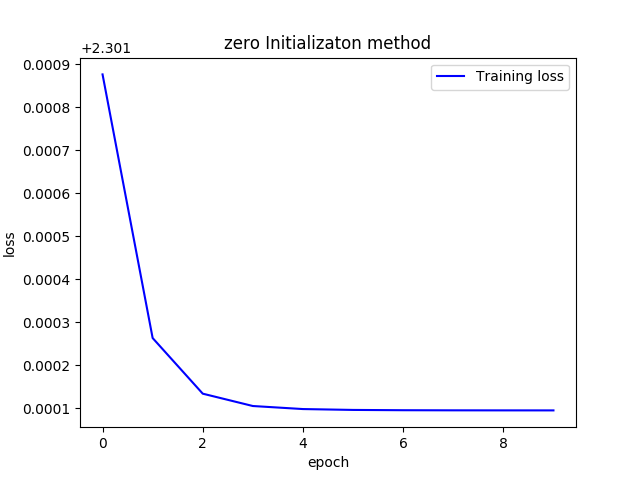
\includegraphics[width=1\textwidth]{zero_init.png}
\caption{\label{fig:init1}average loss against the training time (epoch) using zero initialization method.}
\end{figure}

\begin{figure}
\centering
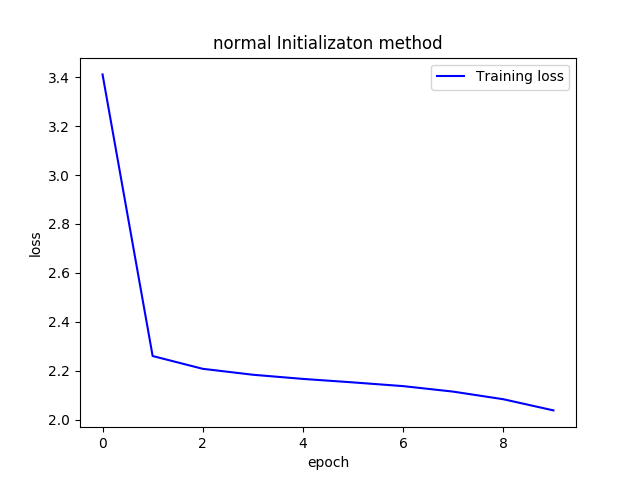
\includegraphics[width=1\textwidth]{normal_init.png}
\caption{\label{fig:init2}average loss against the training time (epoch) using normal initialization method.}
\end{figure}

\begin{figure}
\centering
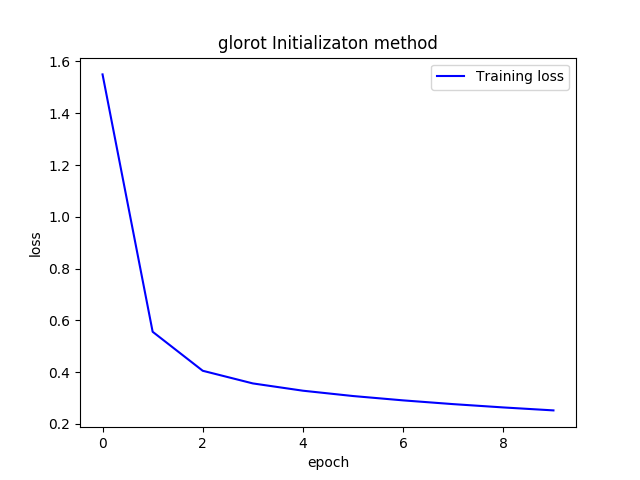
\includegraphics[width=1\textwidth]{glorot_init.png}
\caption{\label{fig:init3}average loss against the training time (epoch) using glorot initialization method.}
\end{figure}

\subsection{Hyperparameter Search}

\begin{enumerate}

\item
The combination of hyper-parameters that we found in which the average accuracy rate on the validation set reach 97.2\% accuracy:
A network with 2 hidden layers h1 = 64 hidden units and h2 = 32 hidden units with a total number of parameters of 52650. A Relu activation function, a learning rate of 0.01, a mini batch size of 64, a number of epochs of 50. (See Figure \ref{fig:lr1} plotting the training/validation accuracy over epochs).

\item 
We tried different hyper-parameters for learning rate, number of epochs {\color{red}{Number of epochs is not an hyperparameter, see slack channel tp1 01/29}}, network architecture and batch size. We consider the same model architecture.

\subsubsection{Learning rate}

We keep the same settings and we only change the learning rate.

\begin{itemize}

\item learning rate of 0.01: validation accuracy = 97.2\% (See Figure \ref{fig:lr1}).

\item learning rate of 0.1: validation accuracy = 97.6\% (See Figure \ref{fig:lr2}).

\item learning rate of 0.001: validation accuracy = 93\% (See Figure \ref{fig:lr3}).  
  
\end{itemize}

\begin{figure}
\centering
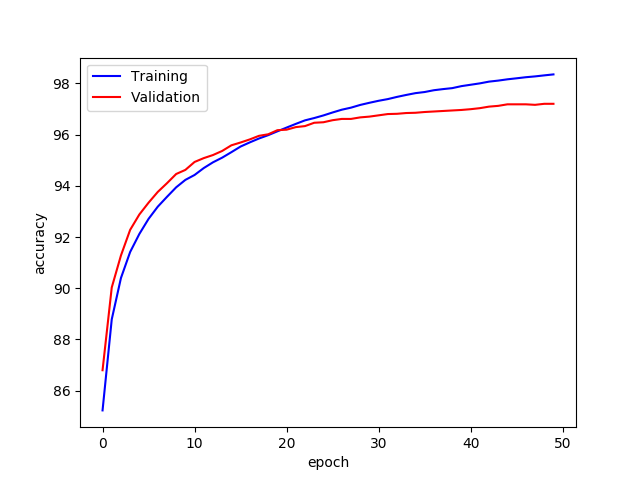
\includegraphics[width=1\textwidth]{acc_hyper.png}
\caption{\label{fig:hyper}Validation/training accuracy against the training time (epoch) using the chosen hyper-parameters.}
\end{figure}

\begin{figure}
\centering
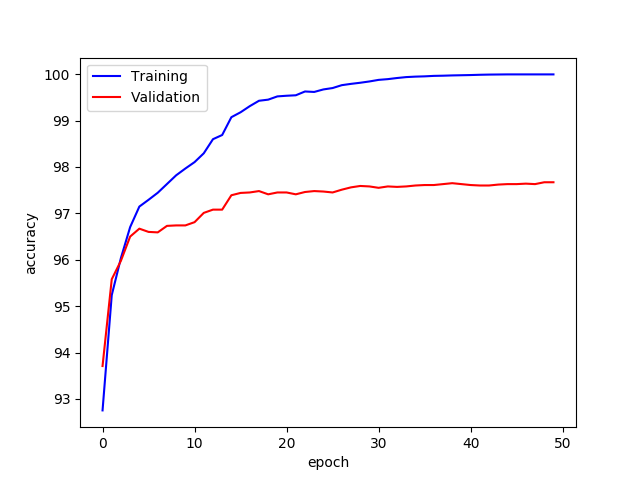
\includegraphics[width=1\textwidth]{lr2.png}
\caption{\label{fig:lr2}Validation accuracy against the training time (epoch) using a learning rate of 0.1.}
\end{figure}

\begin{figure}
\centering
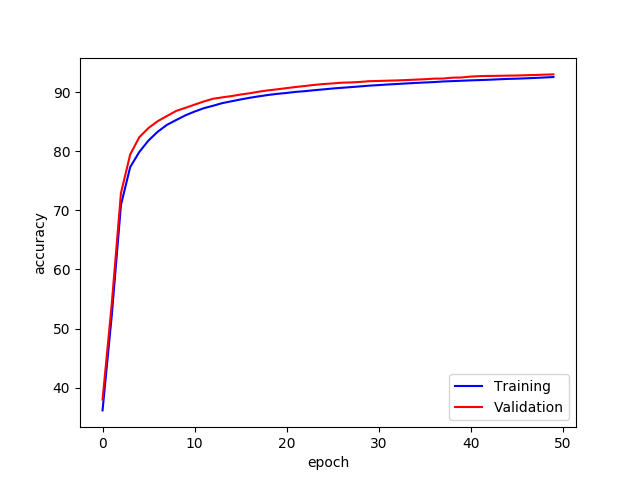
\includegraphics[width=1\textwidth]{lr3.png}
\caption{\label{fig:lr3}Validation accuracy against the training time (epoch) using a learning rate of 0.001.}
\end{figure}


\subsubsection{Number of epochs}
We keep the same settings and we only change the number of epochs.

\begin{itemize}

\item number of epochs of 50: validation accuracy = 97.2\% (See Figure \ref{fig:hyper}).

\item number of epochs of 5: validation accuracy = 92.8\% (See Figure \ref{fig:epoch2}).

\item number of epochs of 150: validation accuracy = 97.3\% (See Figure \ref{fig:epoch3}).  
  
\end{itemize}

\begin{figure}
\centering
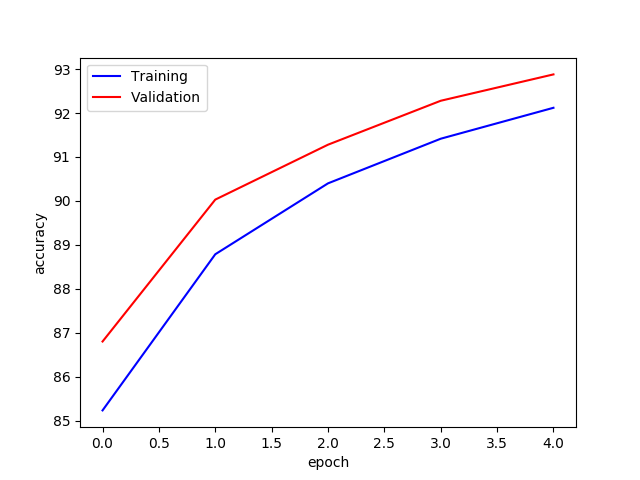
\includegraphics[width=1\textwidth]{epoch2.png}
\caption{\label{fig:epoch2}Validation/training accuracy against the training time (epoch) using a number of epochs of 5..}
\end{figure}

\begin{figure}
\centering
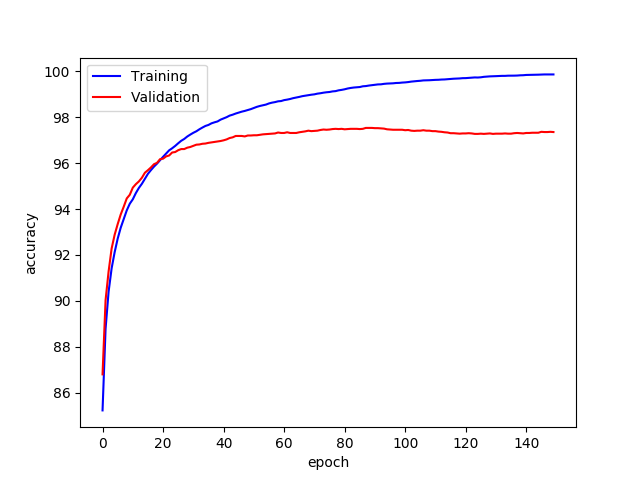
\includegraphics[width=1\textwidth]{epoch3.png}
\caption{\label{fig:epoch3}Validation/training accuracy against the training time (epoch) using a number of epochs of 150.}
\end{figure}

\subsubsection{Number of mini-batches}
We keep the same settings and we only change the number of mini-batches.

\begin{itemize}

\item number of mini-batches of 64: validation accuracy = 97.2\% (See Figure \ref{fig:hyper}).

\item number of mini-batches of 8: validation accuracy = 97.4\% (See Figure \ref{fig:batch2}).

\item number of mini-batches of 512: validation accuracy = 93.4\% (See Figure \ref{fig:batch3}).  
  
\end{itemize}

\begin{figure}
\centering
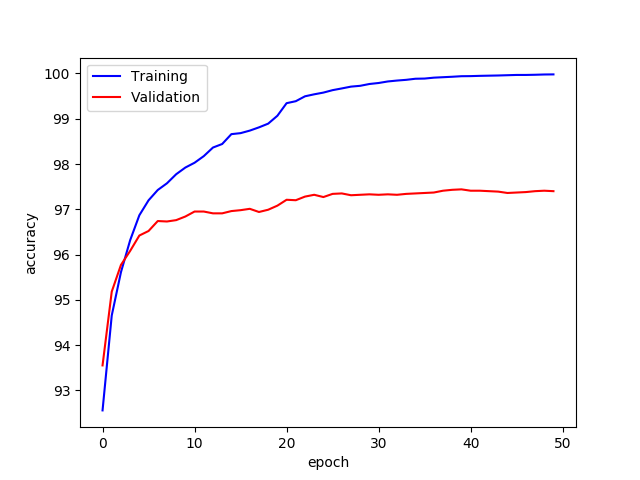
\includegraphics[width=1\textwidth]{batch2.png}
\caption{\label{fig:batch2}Validation/training accuracy against the training time (epoch) using a number of mini-batches of 8.}
\end{figure}

\begin{figure}
\centering
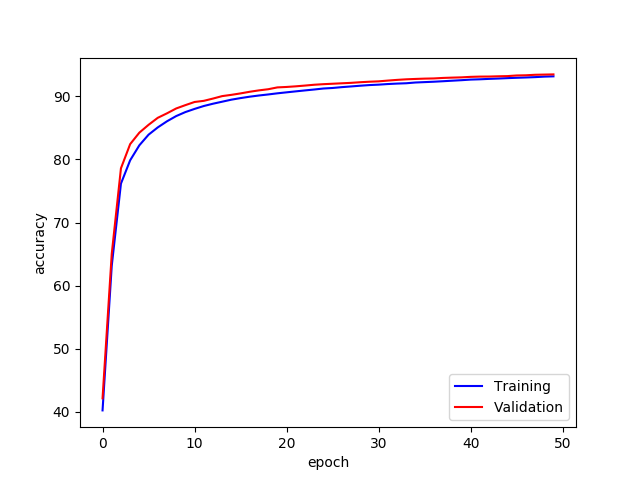
\includegraphics[width=1\textwidth]{batch3.png}
\caption{\label{fig:batch3}Validation/training accuracy against the training time (epoch) using a number of mini-batches of 512.}
\end{figure}

\subsubsection{Non-linearity activation function}
We keep the same settings and we only change the activation function.

\begin{itemize}

\item Relu activation function: validation accuracy = 97.2\% (See Figure \ref{fig:hyper}).

\item Sigmoid activation function: validation accuracy = 92.2\% (See Figure \ref{fig:sigmoid}).

\item tanh activation function: validation accuracy = 93.9\% (See Figure \ref{fig:tanh}).  
  
\end{itemize}

\begin{figure}
\centering
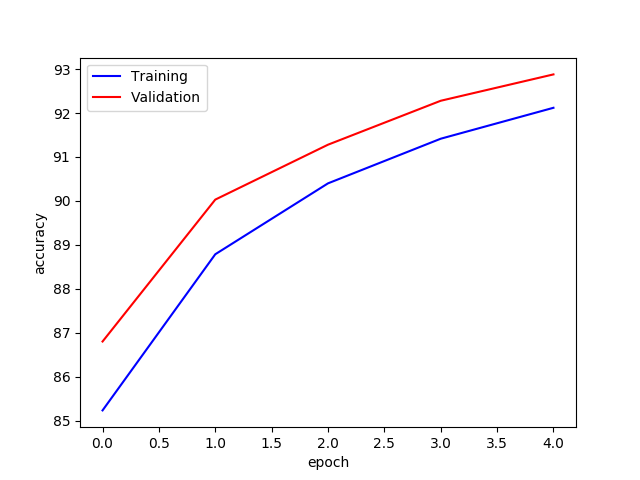
\includegraphics[width=1\textwidth]{epoch2.png}
\caption{\label{fig:sigmoid}Validation/training accuracy against the training time (epoch) using a sigmoid activation function.}
\end{figure}

\begin{figure}
\centering
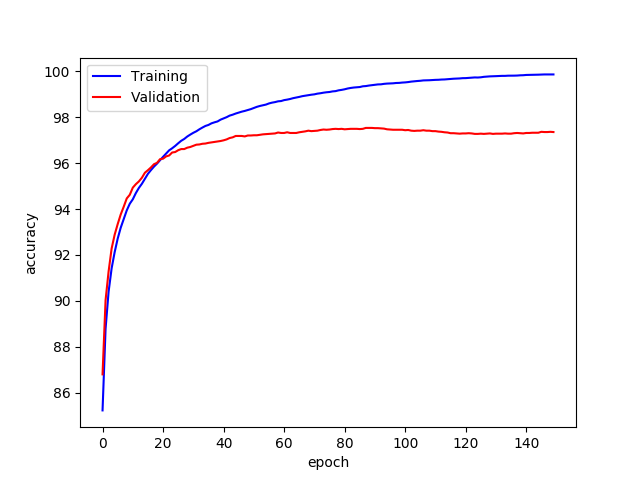
\includegraphics[width=1\textwidth]{epoch3.png}
\caption{\label{fig:tanh}Validation/training accuracy against the training time (epoch) using a tanh activation function.}
\end{figure}

\subsubsection{Network architecture (number of hidden units)}
We keep the same settings and we only change the hidden layers dimensions.

\begin{itemize}

\item Network with 2 hidden layers h1 = 64, h2 = 32: validation accuracy = 97.2\% (See Figure \ref{fig:hyper}).

\item Sigmoid activation function: validation accuracy = 92.2\% (See Figure \ref{fig:lr2}).

\item tanh activation function: validation accuracy = 93.9\% (See Figure \ref{fig:lr3}).  
  
\end{itemize}

\subsection{Gradient validation using finite difference approximation}
We implemented a gradient validation function \emph{grad\_check} which returns the maximum difference between the true gradient and the finite difference gradient approximation for a given number of elements of a network parameter and a given precision $\epsilon$.

We validated the gradients for the first $p=\min(10,m)$ elements of the second layer weights ($W2$) with $m$ number of elements. Using $\epsilon=\frac{1}{N}$ Figure \ref{fig:grad_check} shows the maximum difference as a function of the $N$.

\begin{figure}
\centering
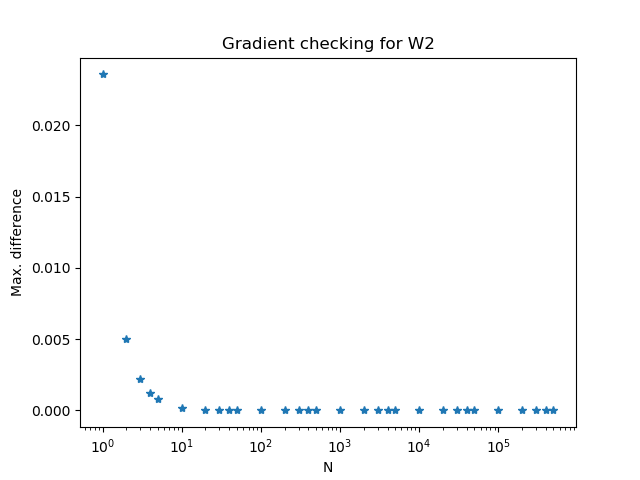
\includegraphics[width=1\textwidth]{grad_check}
\label{fig:grad_check}
\caption{Maximum difference between the analytic gradient and the finite difference approximation for some elements of the weight matrix at the second layer as a function of the precision $N = \frac{1}{\epsilon}$}
\end{figure}

The approximation of the gradient for each element gets closer to the real partial derivative as $\epsilon$ gets smaller, this is consistent with theory since in the definition of the derivative the epsilon tends to zero. 

\end{enumerate}

\section{Problem 2 Convolutional Networks}
\label{sec:problem2}
\subsection{Architecture}
As it is a common practice, we decided to implement our convolutional network using layers that sequentially apply a convolution followed by a ReLU followed by pooling.
Given the size of the images in the dataset MNIST ($28\times28$ pixels) we decided to use four layers where the convolutions are padded in order to keep the size and the pooling kernels have a spatial size $2\times2$ and stride of 2 to obtain a single spatial dimension at the end. In order to fix some other parameters we chose the convolution kernels to have the spatial size of $3\times3$ and the number of channels at to double at each convolution layer. With these settings the only parameter that controls the size of the network is the number of output channels at the first convolutional layer. 

In order to obtain a similar number of parameters than our mlp of Problem~\ref{sec:problem1} ($\sim50K$ parameters) we set that value to $12$, so the number of channels at the layers of our network are  $1,12,24,48,96$. 
\subsection{Performance}
Figure~\ref{fig:CNN_accuracy} shows the training and validation accuracy of the model at each epoch. After training the model for 10 epoch we obtain a validation accuracy of $97\%$

\begin{figure}
\centering
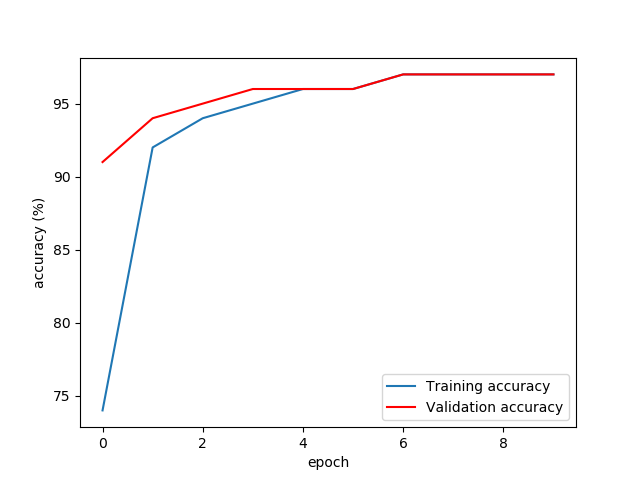
\includegraphics[width=1\textwidth]{P2_CNN_accuracy}
\label{fig:CNN_accuracy}
\caption{Training and validation accuracy of the convolutional model of Section~\ref{sec:problem2}}
\end{figure}



\section{Problem 3 (Kaggle challenge)}
\label{sec:problem3}

\subsection{Architecture of the model}
The model's architecture that we have used is inspired from VGG model, which has the following components (see Figure \ref{fig:vgg}) :

\begin{itemize}
	\item[-] 13 convolutions layers, with 0 padding at each layer, with a kernel of size (3,3) and stride of 1.
	\item[-] 5 max pooling with kernel of size (2,2) and stride of 2.
	\item[-] 2 fully connected layers with 2048 hidden units
	\item[-] 1 output layer
\end{itemize}

%\begin{figure}[h!]
%\centering
%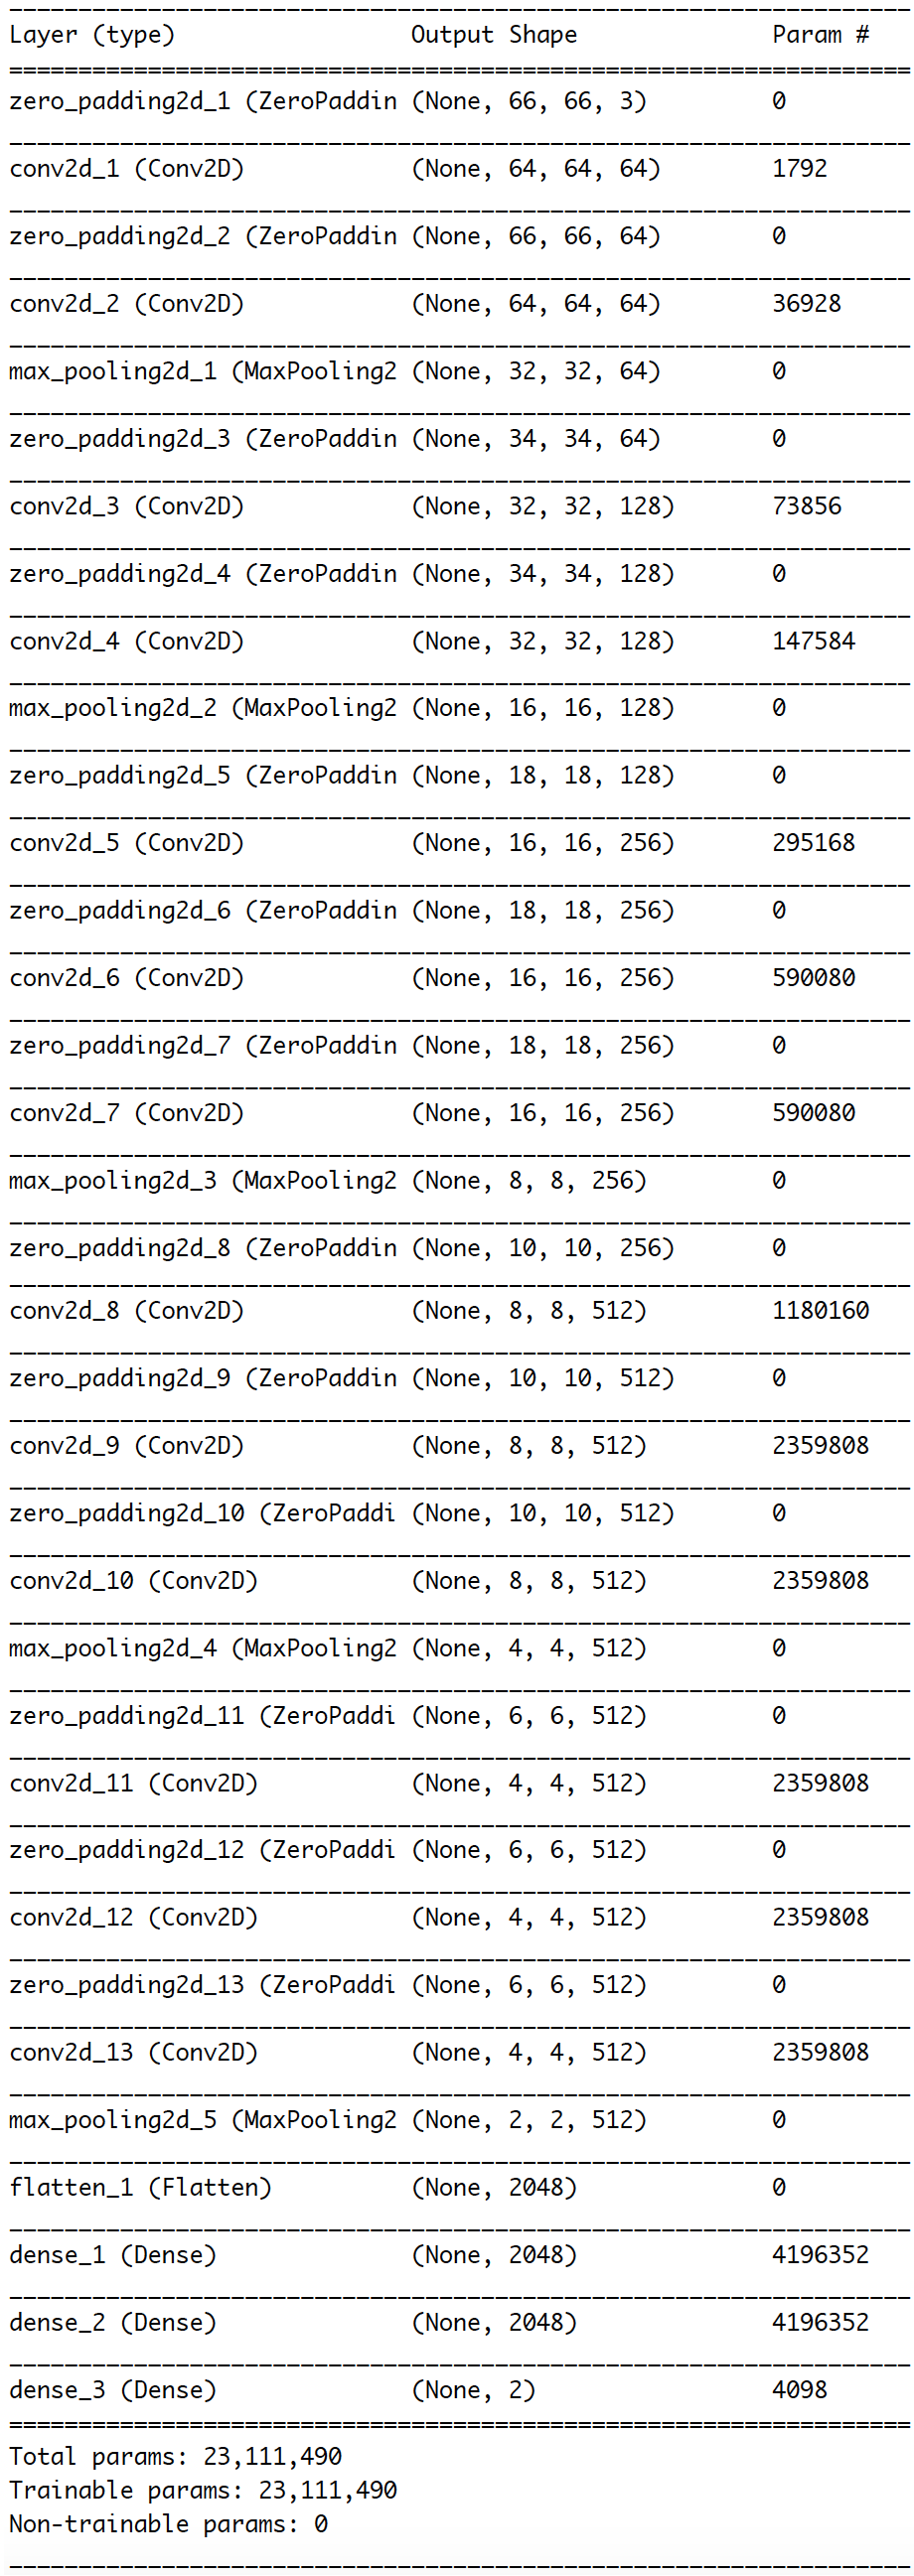
\includegraphics[scale=0.45]{VGG_arch.png}
%\caption{Model architecture}
%\label{fig:vgg}
%\end{figure}

The total parameters of this model is 23,111,490, which is a medium size in comparison of the more recent deep models.

It worth saying that our experimentation has shown that a model with more layers performs better than a model with a fewer ones. In fact, for this competition, we have found that the VGG model above have performed better than AlexNet-based architecture.

\subsection{Learning curves}
The following figures (\ref{fig:vggloss},\ref{fig:vggacc}) show respectively the training and validation loss and accuracy by epochs:

\begin{figure}[h!]
	\centering
	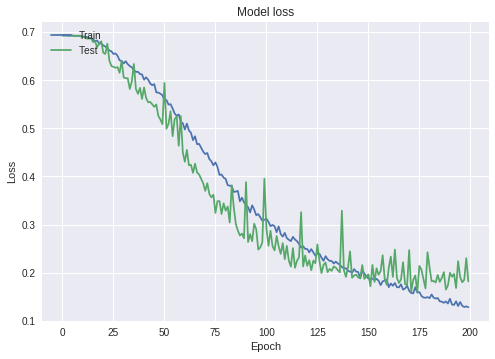
\includegraphics[scale=.6]{VGGLoss_of.png}
	\caption{Loss of the model by epoch}
	\label{fig:vggloss}
\end{figure}

\begin{figure}[h!]
	\centering
	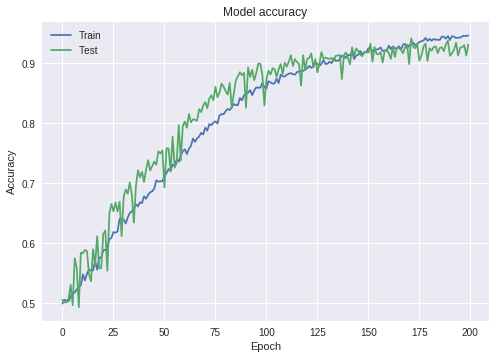
\includegraphics[scale=.6]{VGGAccu_of.png}
	\caption{Accuracy of the model by epoch}
	\label{fig:vggacc}
\end{figure}

Before starting training the model, we have split the input images randomly to training and validation sets with a ratio of $80\%-20\%$ respectively. (see the code on appendix).

We have also used data augmentation strategy to improve the variance of the model.

The learning curves show that the model has a high bias and high variance at the beginning of the training and then starts learning till an optimal value around 150 epochs. After that point, the model starts overfitting as the accuracy and loss on the training set was bigger than those on the validation set.


\begin{figure}[h!]
	\centering
	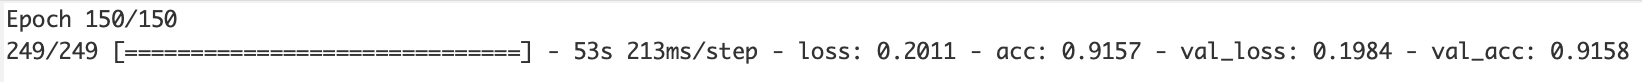
\includegraphics[scale=.5]{150epoch.png}
	\caption{Accuracy and Loss after 150 epochs}
	\label{fig:150epoch}
\end{figure}


We believe that a regularization strategy as \textit{Weight decay} could potentially get a better result, as it will push the model to learn beyond 150 epochs without overfitting.

Notice that the accuracy on the testset is better than the accuracy on the validation set, which is a proof that the model generalize well, and the data augmentation strategy was a good one to improve the model's performance on unseen data.

\subsection{Hyperparameters settings}
We have selected different hyperparameters to tune on the validation set in order to get the best model configuration, which are:
- Number of hidden layers
- Size of the kernels
- Learning rate
- Batch size

The following table gives a comparison of the model's performance while for each parameter while keeping the others fixed.

The table below (\ref{table:1}) show the accuracy of the model for given different model architecture while keeping fixed the other parameters : kernel size, number of epoch, ...

\begin{table}[h!]
	\centering
	\begin{tabular}{||c c c c||} 
		\hline
		Nbr of layers & Accuracy & Loss & Total nb of parameters\\ [0.5ex] 
		\hline\hline
		6 & 0.3109 & 0.8574 & 2,736,066\\ 
		10 & 0.2713 & 0.8841 & 5,147,458\\ 
		13 & 0.2068 & 0.9078 & 17,076,546\\ 
		16 lite & 0.1984 & 0.9158 & 23,111,490\\ 
		16 & ? & ? & 39,896,898\\  [1ex] 
		\hline
	\end{tabular}
	\caption{Number of layers tuning}
	\label{table:1}
\end{table}

We notice that a model has a better performance when he has more hidden layers. This is normal because more layers means more capacity for the model.

The next table (\ref{table:2}) gives a comparison for different kernel size. This hyperparameter influence drasticly the architecture of the model, that is a bigger kernel shorten the model and it could'nt be deeper unless we add 0 padding which gives a poorer feature map. We notice that in general a smaller kernel size gives a better result!

\begin{table}[h!]
	\centering
	\begin{tabular}{||c c c||} 
		\hline
		Kernel size & Accuracy & Loss \\ [0.5ex] 
		\hline\hline
		2 & 0.5832 & 0.6919 \\ 
		3 & 0.5761 & 0.6912 \\ 
		4 & 0.5444 & 0.6894 \\ 
		5 & 0.5418 & 0.6930 \\ [1ex]  
		\hline
	\end{tabular}
	\caption{Kernel size tuning}
	\label{table:2}
\end{table}

The next table (\ref{table:3}) gives a comparison of the model performance as a function of the batch size. We notice that a small batch size push the model to make more iterations which make the SGD converge better than with bigger batch size.

\begin{table}[h!]
	\centering
	\begin{tabular}{||c c c||} 
		\hline
		Batch size & Accuracy & Loss \\ [0.5ex] 
		\hline\hline
		16 & 0.5320 & 0.6892 \\ 
		32 & 0.5015 & 0.6919 \\ 
		64 & 0.4859 & 0.6935 \\ 
		128 & 0.5000 & 0.6929 \\ [1ex]  
		\hline
	\end{tabular}
	\caption{Kernel size tuning}
	\label{table:3}
\end{table}

And finally, table (\ref{table:4}) gives a comparison of the model performance as a function of the learning rate. We notice, that the model convergence is very slow with a small learning rate and faster with a relatively bigger one like 0.03.

\begin{table}[h!]
	\centering
	\begin{tabular}{||c c c||} 
		\hline
		Learning rate & Accuracy & Loss \\ [0.5ex] 
		\hline\hline
		0.03 & 0.8935 & 0.2417 \\ 
		0.01 & 0.8595 & 0.3279 \\ 
		0.003 & 0.6930 & 0.5981 \\
		0.001 & 0.5825 & 0.6709 \\ [1ex]  
		\hline
	\end{tabular}
	\caption{Kernel size tuning}
	\label{table:4}
\end{table}

Our final model has those values as hyperparameters:
- Number of hidden layers: 13 convolutions and 3 FC
- Size of the kernels: (3,3)
- Learning rate: 0.03
- Batch size: 16

This model give an accuracy of : $94\%$ on validation set and $93.7\%$ on the public leaderboard. The model was trained for 200 but get his best parameters around 150 epochs.

As we haven't used any regularization strategies, on the training phase, we have used the early stopping strategy the use the best model's parameters before he starts overfitting.

The model get a decent performance (not expected though) of $91\%$ on validation set and $92\%$ (see Figure \ref{fig:150epoch} on the public leader board (see Figure \ref{fig:kaggle}) which is a very good result.

\begin{figure}[h!]
	\centering
	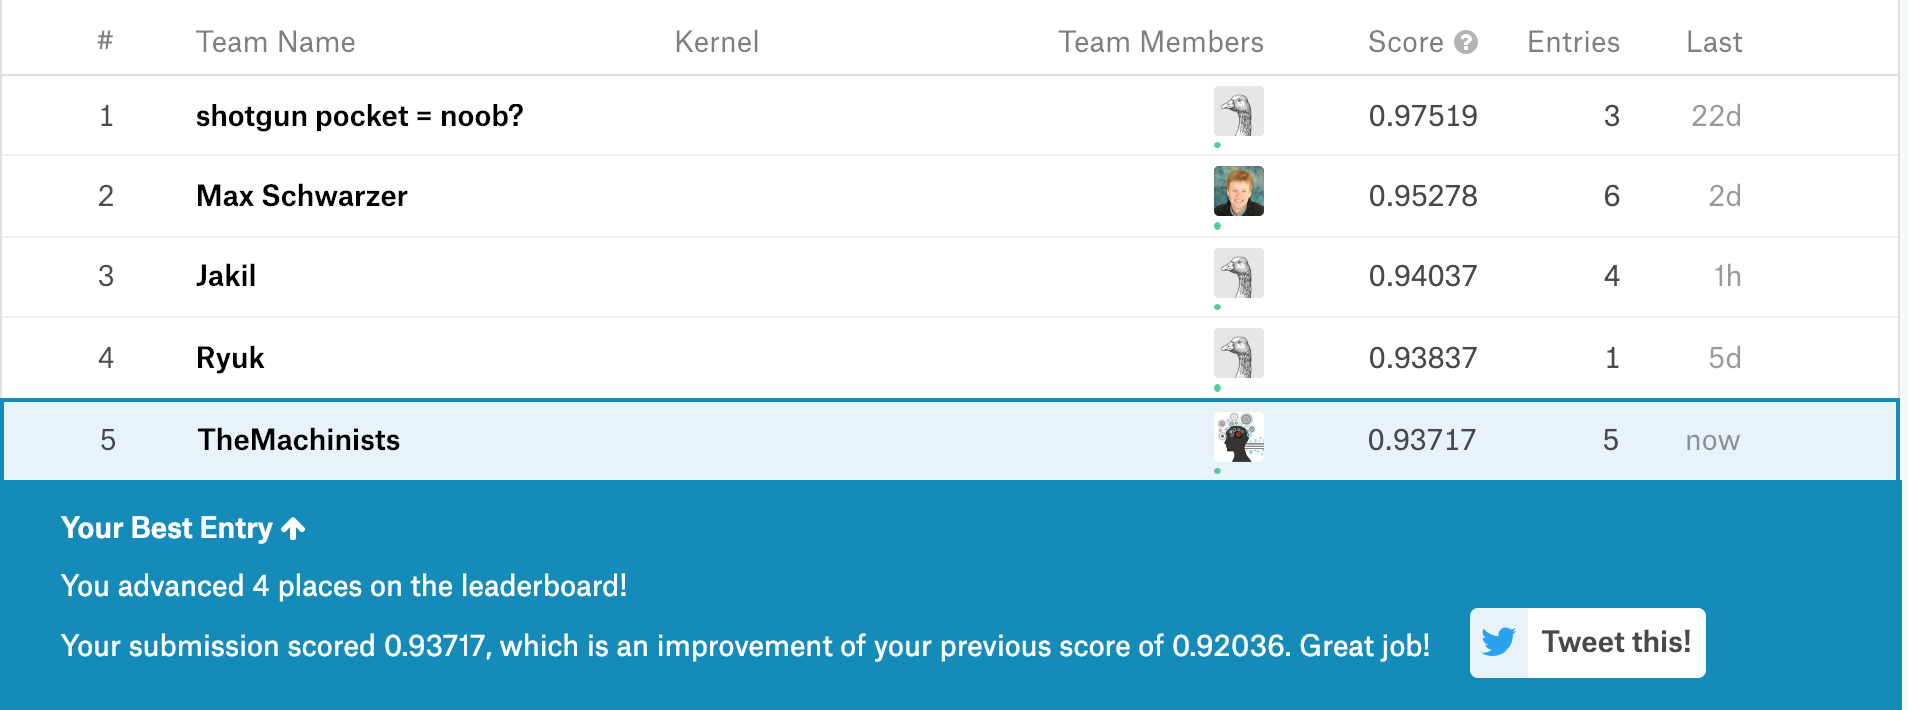
\includegraphics[scale=.4]{kaggle.png}
	\caption{Rank at the public leaderboard}
	\label{fig:kaggle}
\end{figure}

\subsubsection{Feature map visualization}
The feature map visualization give in some sens an intuition on how a CNN works to learn from images. Across the layers, the feature map go from high level pattern recognition to low level as we go deeper in the model. The following image shows for each layers the feature map after each activation layer

\begin{figure}[h!]
	\centering
	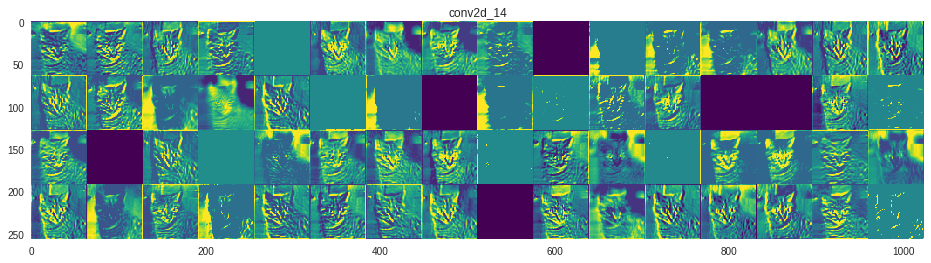
\includegraphics[scale=.3]{fp1.png}
	\caption{Feature map after conv layer 1}
	\label{fig:fp1}
\end{figure}

\begin{figure}[h!]
	\centering
	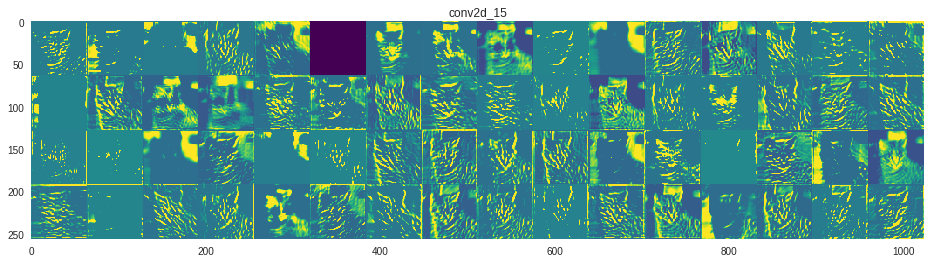
\includegraphics[scale=.3]{fp2.png}
	\caption{Feature map after conv layer 2}
	\label{fig:fp2}
\end{figure}

\begin{figure}[h!]
	\centering
	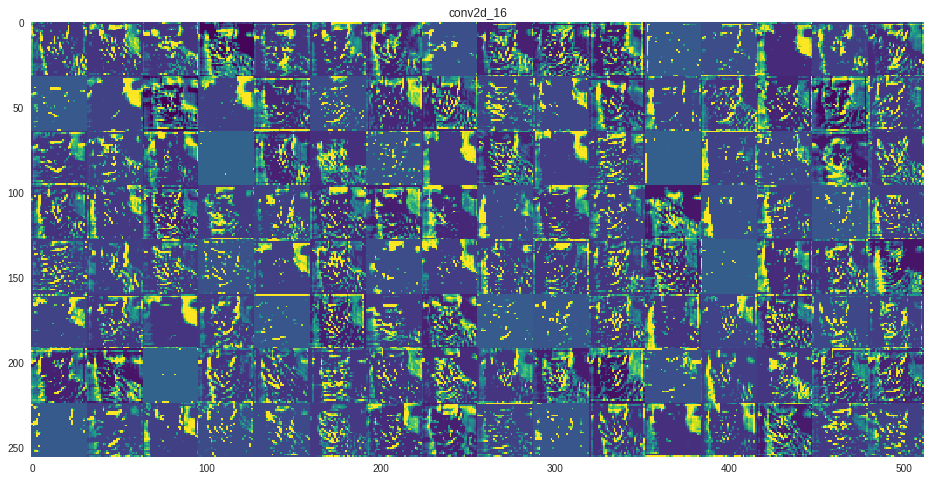
\includegraphics[scale=.3]{fp3.png}
	\caption{Feature map after conv layer 3}
	\label{fig:fp3}
\end{figure}

\subsubsection{Performance of the model}
The model get nearly $94\%$ accuracy on test set (public leaderboard) which is not bad given that we haven't used any fancy techniques like regularization. It is interesting to see, what kind of images the model has misclassified. The following images are examples of Cats that the model has classified to Dogs:


Here some images that the model predict around 50\%:


Here some examples where the images are 
(a) clearly misclassified

(b) where the classifier predicts around 50\% on both classes.  

Explain your observation and/or suggest any improvements you think may help.

\begin{thebibliography}
@online{,
  author = {Thayumanav Jayadevan},
  title = {Why don't we initialize the weights of a neural network to zero?},
  year = 2018,
  url = {https://www.quora.com/Why-dont-we-initialize-the-weights-of-a-neural-network-to-zero},
  urldate = {2019-02-05}
}
\end{thebibliography}
\end{document}